\documentclass{beamer}

\usepackage{listings}
\usepackage{tabulary}
\usepackage[utf8]{inputenc}
\usetheme{Madrid}
\setbeamersize{text margin left=0.1\textwidth,text margin right=0.1\textwidth}
\setbeamertemplate{section in toc}{\inserttocsection}
\lstset{language=python,
        keywordstyle=\color{red},
        basicstyle=\ttfamily,
        basicstyle=\small,
        frame = single,
        framexleftmargin=15pt,
        numbers=left, 
        numberstyle=\small, 
        numbersep=5pt, 
        xleftmargin=0.05\textwidth,
        columns=fullflexible}

%Information to be included in the title page:
\title{Hadoop}
\subtitle{Introduction to Distributed Systems and MapReduce}
\author{Cary Goltermann}
\institute{Galvanize}
\date{2016}

\AtBeginSubsection[]
{
  \begin{frame}
    \frametitle{Overview}
    \tableofcontents[currentsection,currentsubsection]
  \end{frame}
}
 
\begin{document}
 
\frame{\titlepage}
 
\begin{frame}
  \frametitle{Overview}
  \tableofcontents[]
\end{frame}

\section{Big Data}
\subsection{What is it and Why is it Important?}
\begin{frame}
  \frametitle{Big Data}
  \centering
  \underline{\LARGE The Three Vs}
  \vspace{6mm}
  \begin{block}{}
    {\large ``Big data is \textbf{high volume}, \textbf{high velocity}, and/or \textbf{high variety} information assets that require new forms of processing to enable enhanced decision making, insight discovery and process optimization.''}
    \vspace{5mm}
    \hspace*\fill{\small--- Gartner Inc.}
  \end{block}
\end{frame}

\begin{frame}
  \frametitle{3 Vs of Big Data}
  \begin{description}
    \item [High Volume] Data so large that it can't be worked with on a single computer.
    \item [High Velocity] Data input/output too quick for it to be processed by a single computer.
    \item [High Variety] Data in many different, disparately or not at all, structured formats. E.g. text, log file, video, etc.
  \end{description}
\end{frame}

\begin{frame}
  \frametitle{How Big is BIG?}
  \begin{columns}
    \column{\dimexpr\paperwidth-10pt}
    \small
    \begin{tabulary}{\textwidth}{|CC|C|L|L|L|}
      \hline
      \textbf{Class} & &\textbf{Size} & \textbf{Tools} & \textbf{Storage} & \textbf{Examples} \\
      \hline
      Small & & $< 10 GB$ & R / Python & Fits in a single machine's memory & Thousands of sales figures \\ 
      \hline
      Medium & & $10 GB - 1 TB$ & Python w/ indexed files, large database & Fits on a single machine's disk & Millions of web pages \\ 
      \hline
      Large & & $ > 1 TB$ & Hadoop, Spark, distributed databases & Stored across multiple machines & Billion of web clicks \\ 
      \hline
    \end{tabulary}
  \end{columns}
\end{frame}

\begin{frame}
  \frametitle{Why Does Any of This Matter?}
  \begin{center}
    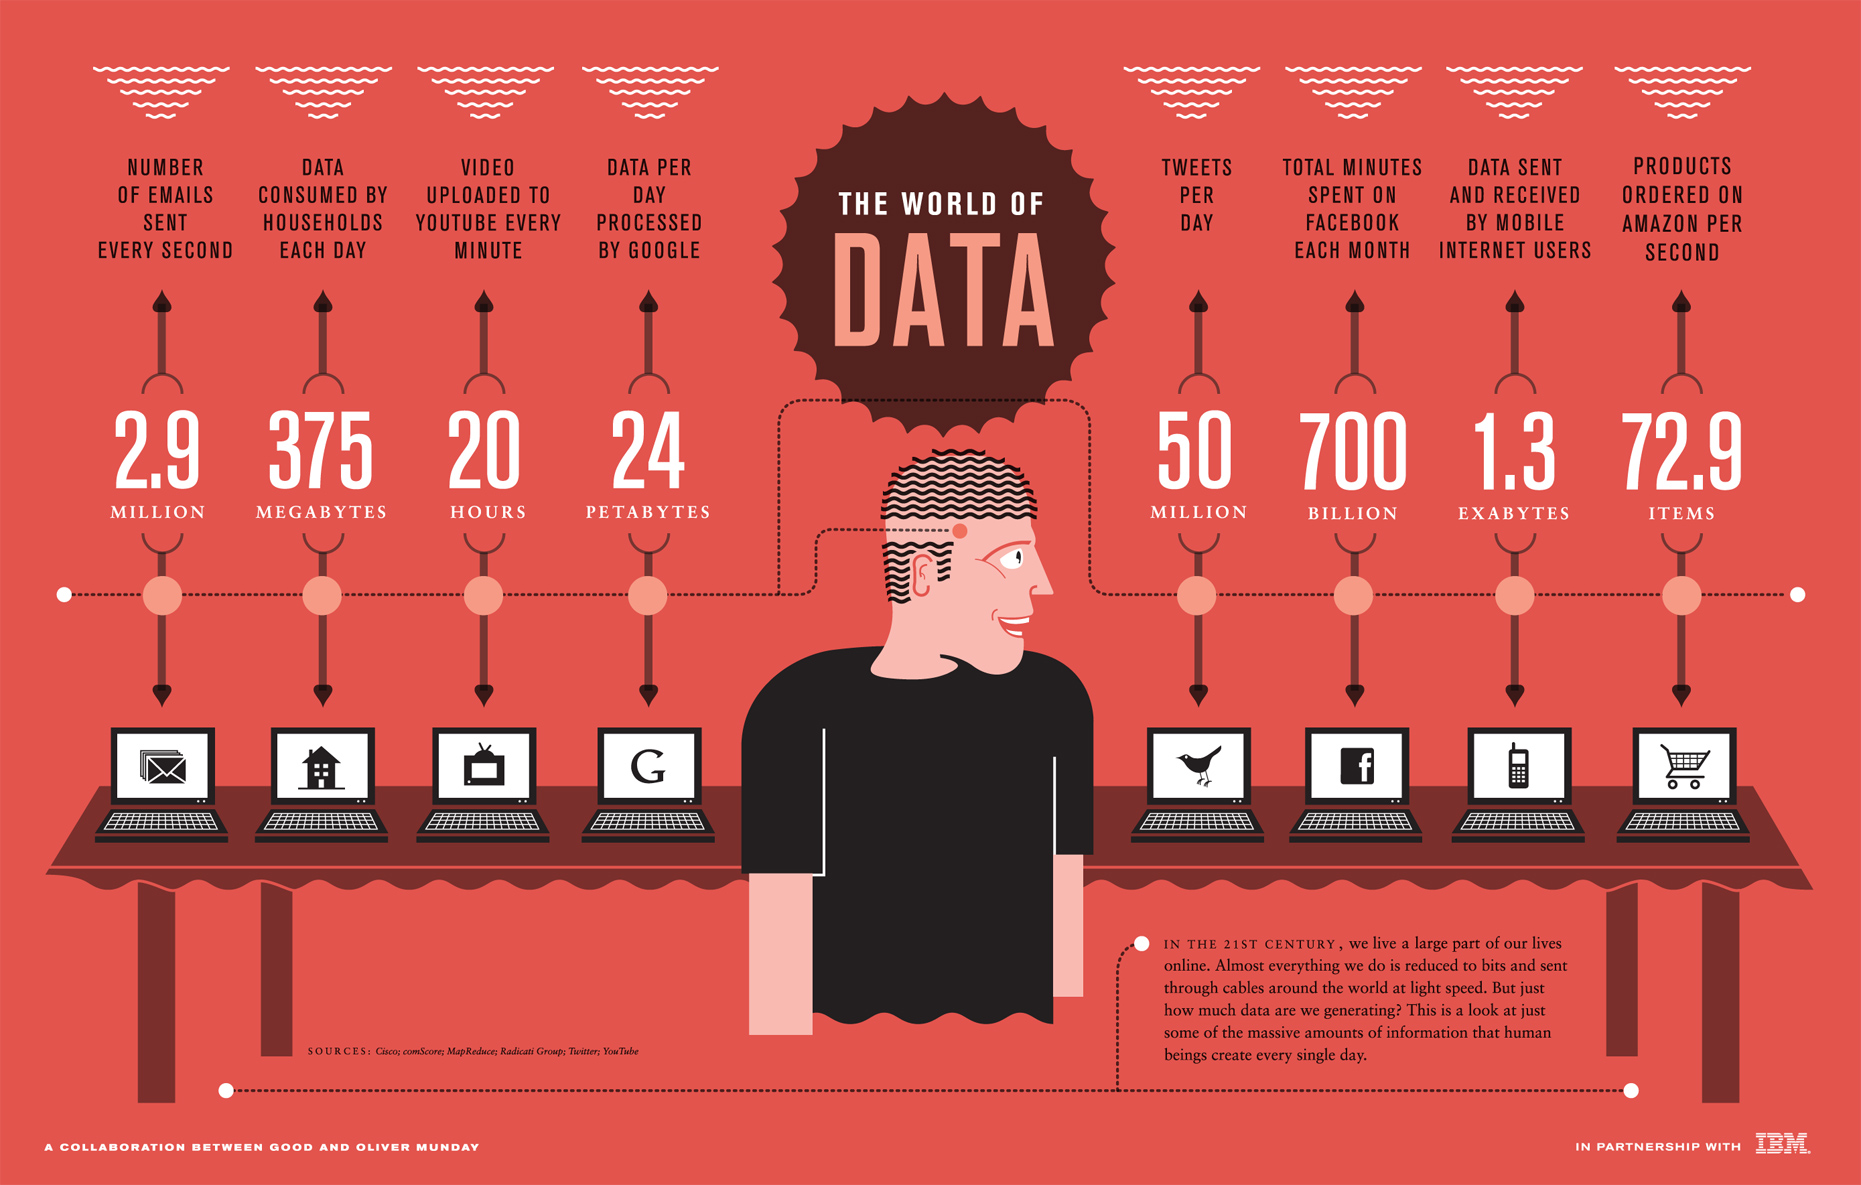
\includegraphics[width=0.7\textwidth]{../images/world_of_data.jpeg}
  \end{center}
  \begin{itemize}
    \item As more data is generated, and inevitably collected, the size of data you'll likely work with is going to increase.
    \item Tools to store and process these larger data sets are going to be increasingly required.
  \end{itemize}
\end{frame}

\section{Distributed Systems}
\begin{frame}
  \frametitle{Local vs. Distributed}
  \begin{columns}
    \column{0.3\textwidth}
      \centering
      
\includegraphics[width=0.6\textwidth]{../images/single_machine.png} \vspace{5mm}

      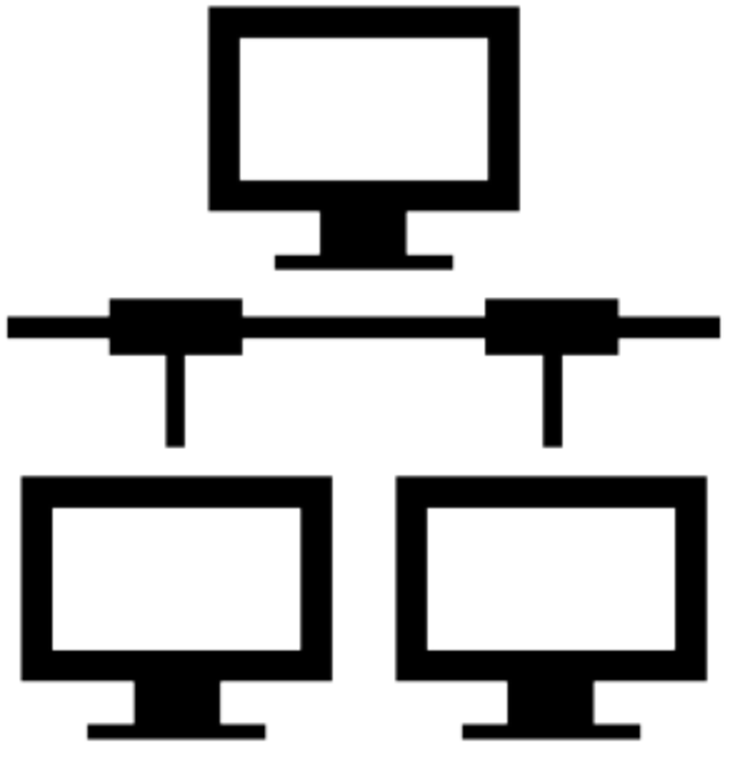
\includegraphics[width=0.7\textwidth]{../images/distributed.png}
    \column{0.6\textwidth}
    \begin{description}
      \item[Local] Use resources of one machine. Does not need to communicate with any others.
      \item[Distributed] Uses the resources, processing and memory, of multiple machines. However, they need to be able to communicate with one another.
    \end{description}
  \end{columns}
\end{frame}

\subsection{Distributed Filesystems and Processing}
\begin{frame}
  \frametitle{Scaling}
  \hspace{2mm}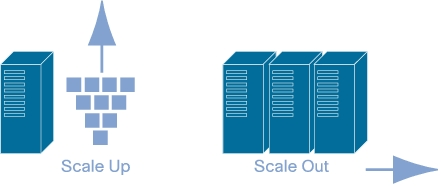
\includegraphics[width=\textwidth]{../images/scaling.jpg}
  \vspace{2mm}
  \begin{columns}
    \column{0.45\textwidth}
    Make the computer bigger:\\ disk, RAM, CPU cores.
    \column{0.55\textwidth}
    Add more computers:\\take advantage of parallelizable algorithms.
  \end{columns}
\end{frame}

\begin{frame}
  \frametitle{Local vs. Distributed: Pros \& Cons}
    {\LARGE \underline{Local}}
    \vspace{1mm}
    \begin{description}
      \item[Pros] Simple, fast when computations are small enough.
      \item[Cons] Physical limits to memory, disk space and CPU power.
    \end{description}
    \vspace{4mm}
    {\LARGE \underline{Distributed}}
    \vspace{1mm}
    \begin{description}
      \item[Pros] Easily linearly scalable, can designed to be fault-tolerant.
      \item[Cons] Slow to communicate over network, need to solve problems with parallelizable techniques.
    \end{description}
\end{frame}

\begin{frame}
  \frametitle{Should I Use Distributed Computing Solutions?}
  \begin{itemize}
    \item Because of the overhead involved with having multiple computers in a network communicate with each other, and the restrained set of problems that can readily be solved in a parallelizable way, it's not a good enough reason to choose a distributed solution just because things are ``taking awhile'' on your local machine.
    \item However, if you'd like to get practice with the Big Data tools so that you feel comfortable with them and can have them on your resume, then it may be worthwhile to use these solutions, even on data this isn't ``\alert{Big}''.
  \end{itemize}
\end{frame}

\subsection{Distributed Systems Architecture}
\begin{frame}
  \frametitle{High Level Architecture}
  \centering
  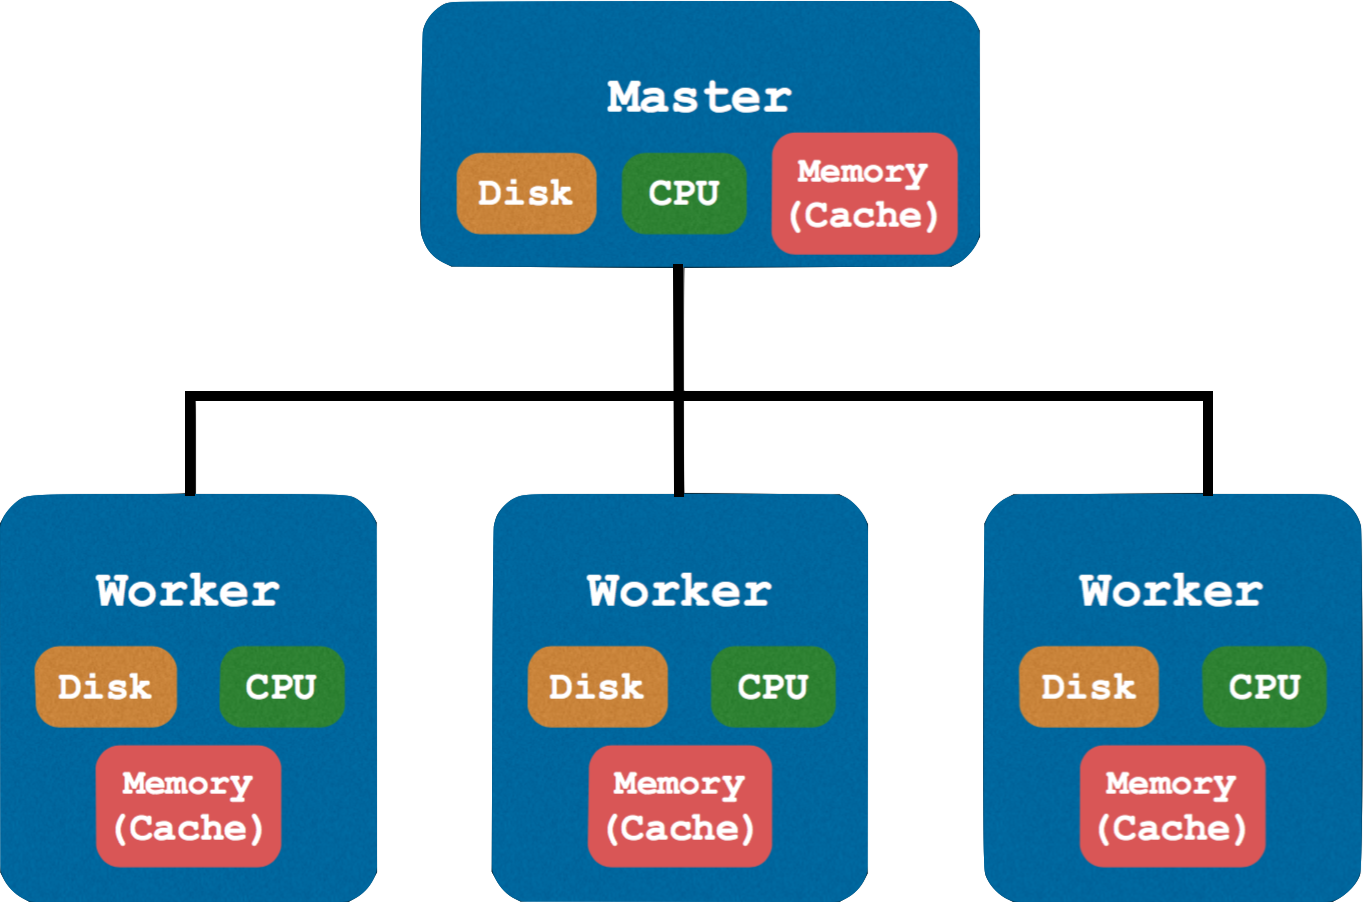
\includegraphics[width=\textwidth]{../images/simple_architecture.png}
\end{frame}

\section{Hadoop}
\subsection{HDFS}
\begin{frame}
  \frametitle{Hadoop Distributed File System Architecture}
  \centering
  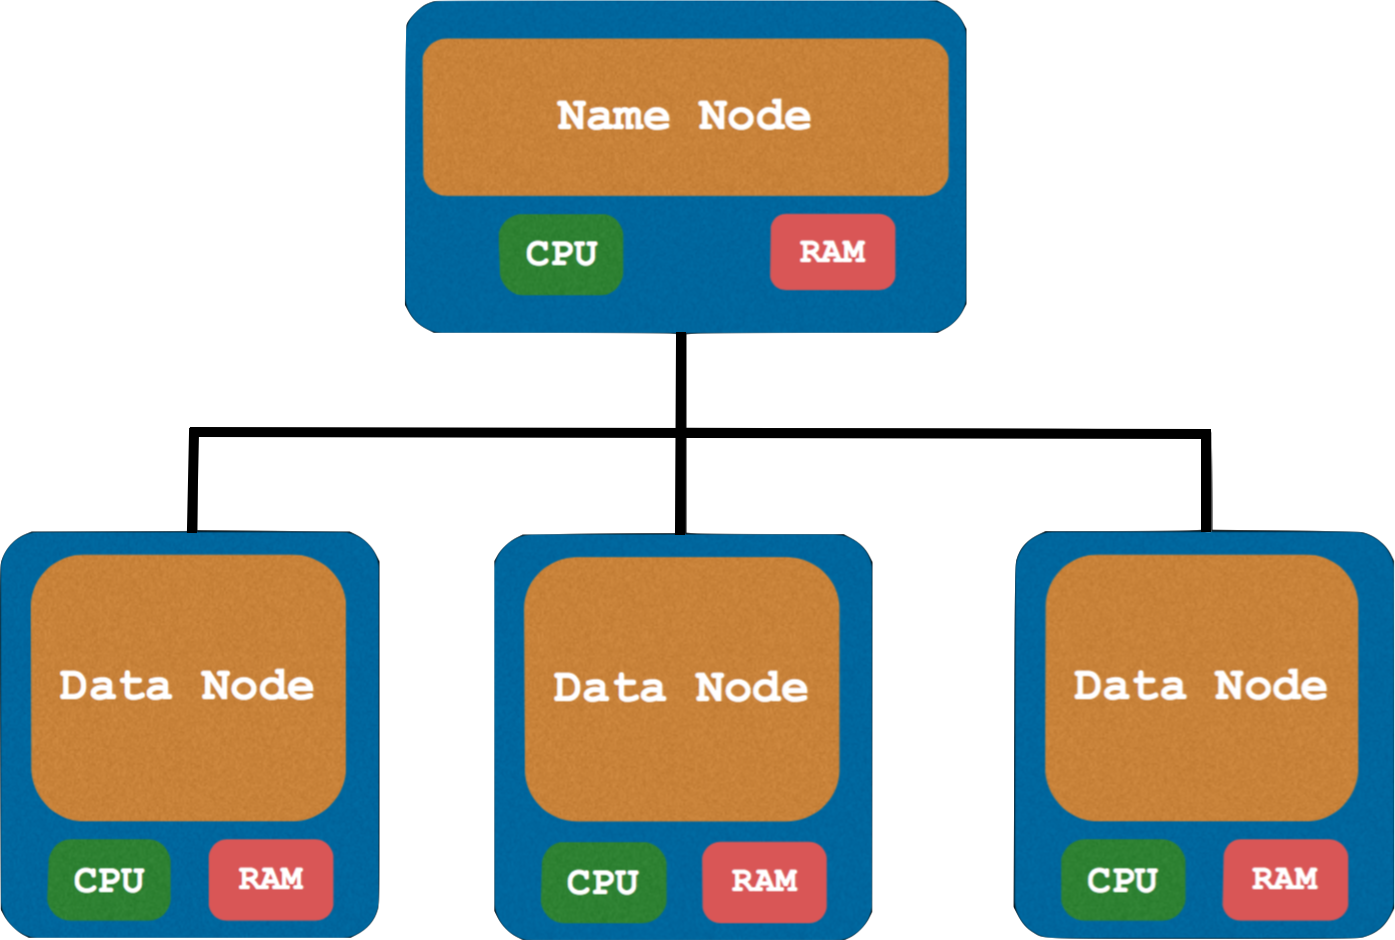
\includegraphics[width=0.8\textwidth]{../images/hdfs_architecture.png}
  \vspace{5mm}
  \begin{columns}
    \column{0.5\textwidth}
    Data nodes store the data.
    \column{0.5\textwidth}
    The name node keeps track of where the data is stored.
  \end{columns}
\end{frame}

\begin{frame}
  \frametitle{Fault-tolerance Through Replication}
  \begin{itemize}
    \item Each file is broken up into blocks, default size is 64/128 MB.
    \item Each of these blocks is replicated on 3, by default, of the data nodes in the cluster.
  \end{itemize} \pause
  \vspace{3mm}
  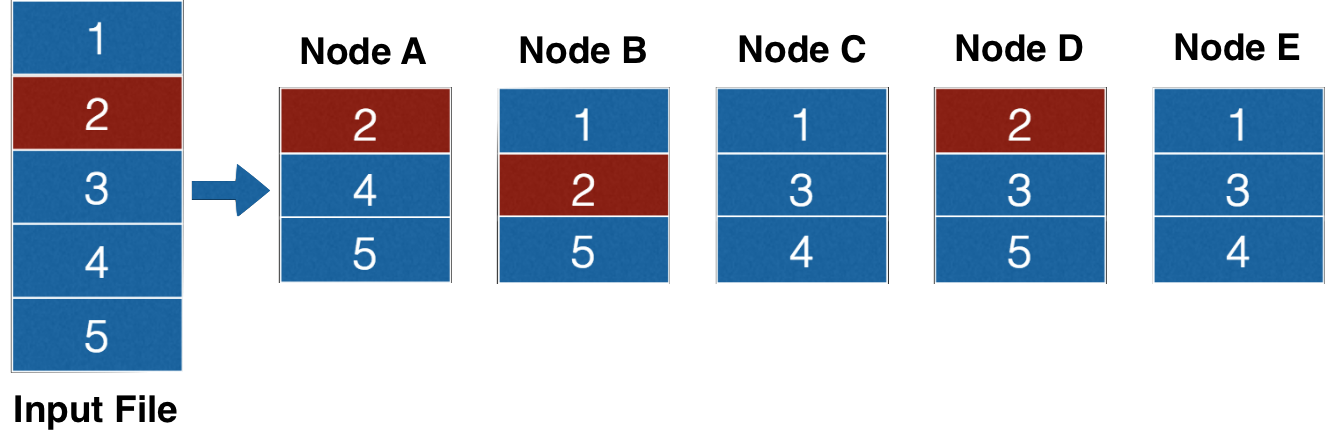
\includegraphics[width=\textwidth]{../images/replication.png}
  \vspace{1mm}
\end{frame}

\begin{frame}
  \frametitle{Question}
  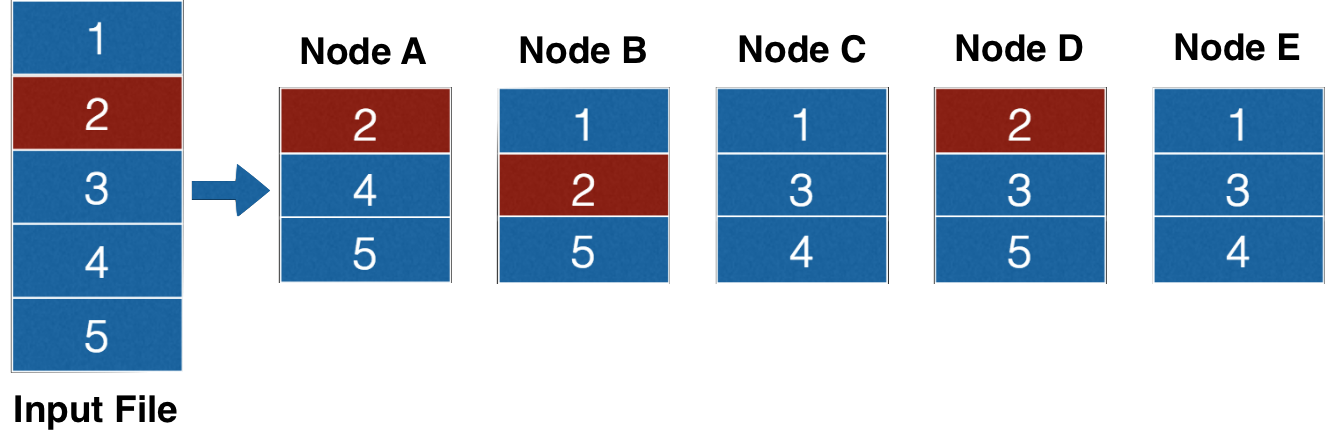
\includegraphics[width=\textwidth]{../images/replication.png}
  \begin{block}{}
    How many nodes can be lost before the original file isn't recoverable?
  \end{block}
\end{frame}

\begin{frame}
  \frametitle{HDFS}
  \centering
  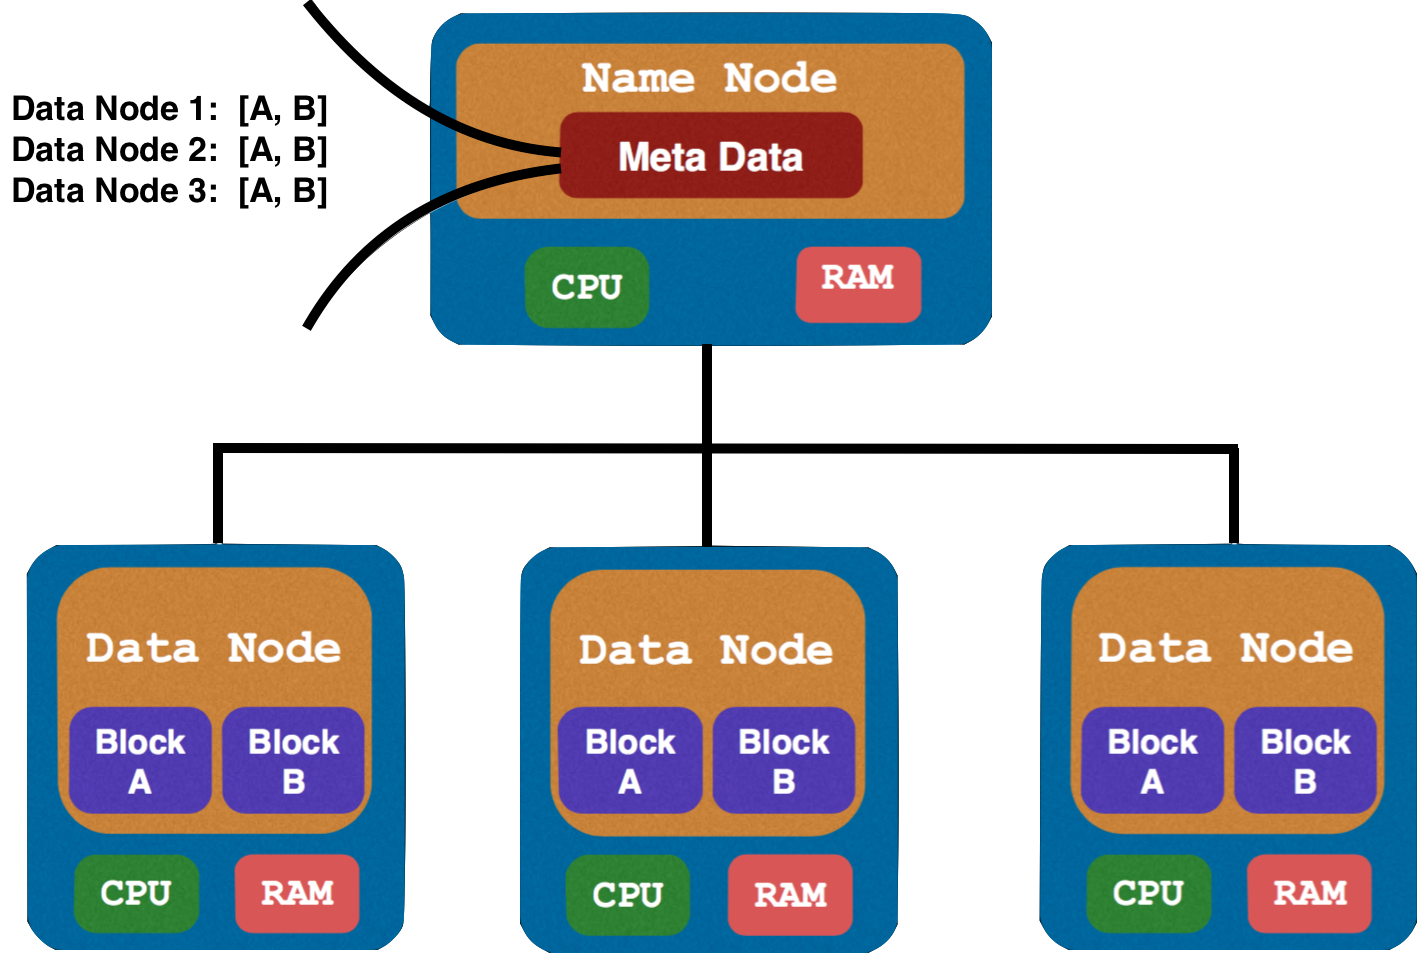
\includegraphics[width=0.8\textwidth]{../images/name_node.png}

  \vspace{4mm}
  \parbox{\linewidth}{Since the name node knows about where all the copies of each block is it can automatically make new ones if some are lost.}
\end{frame}

\subsection{MapReduce}
\begin{frame}
  \frametitle{Processing in Hadoop}
  If HDFS is the storage in our distributed system, then how are would we design a means by which we can process all of our distributed data? \pause
  \vspace{4mm}
  \begin{block}{}
    We can move the computation portion of our endeavors to the computer that is storing each part of our data in HDFS.
  \end{block} \pause
  \vspace{4mm}
  This requires us to have a processing framework which can natively work on data that isn't all stored in the same location. 

  \vspace{4mm}
  \centering   
  Enter \alert{\LARGE MapReduce} ({\LARGE duce...}{\large duce...}{\small duce}).
\end{frame}

\begin{frame}
  \frametitle{Advantages of MapReduce}
  There are a lot of details that need to be taken care of when doing distributed processing:
  \begin{itemize}
    \item Splitting up data
    \item Moving data between nodes
    \item Managing resources, computational and memory
    \item Status and monitoring
    \item Fault-tolerance
  \end{itemize} \pause

  \vspace{4mm}
  MapReduce is automatically going to take care almost all the complications associated with these. All we have to do is play by its rules.
\end{frame}

\begin{frame}
  \frametitle{MapReduce Strategy}
  The intuition of the MapReduce framework boils down to divide and conquer.

  \vspace{4mm}
  \begin{enumerate}
    \item Split a task into smaller subtasks.
    \item Solve these independently of one another (in parallel).
    \item Recombine the output of each subtask into a final result.
  \end{enumerate}
\end{frame}

\begin{frame}
  \frametitle{The Real Map \& Reduce}
  Mapping and reducing are concepts that belong to the functional programming paradigm. They are composed of the:

  \vspace{4mm}
  \begin{description}
    \item[Map] Applies a function to each of the elements of a data structure.
    \item[Reduce] Takes a function which aggregates the elements of a data structure.
  \end{description}

  \vspace{4mm}
  This strategy is particularly useful in distributed computing because the elements of the data structure referenced in the map step don't need to be on the same machine, they can be the partitions of a file that live on different data nodes.
\end{frame}

\begin{frame}
  \frametitle{MapReduce Diagram}
  \centering
  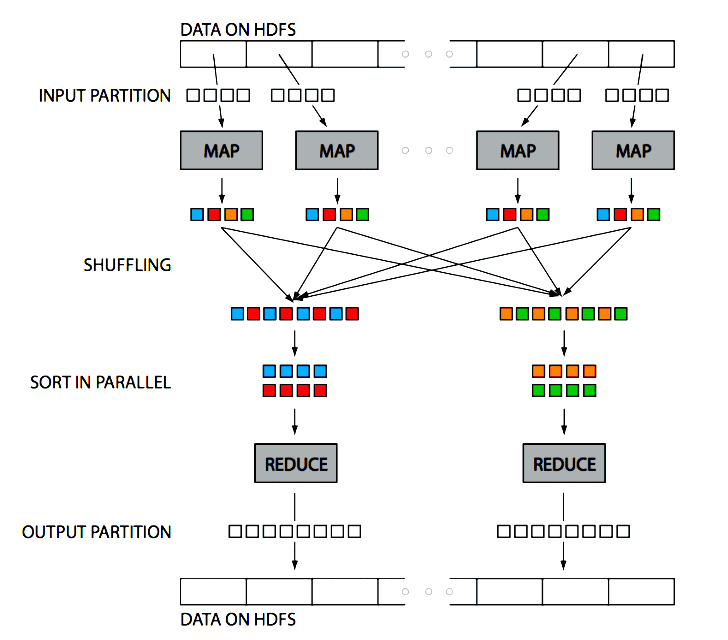
\includegraphics[width=0.7\textwidth]{../images/shuffle_sort.png}
\end{frame}

\begin{frame}
  \frametitle{Map Step}
  Mapping is simply the action of taking in some form of data and filter/transforming it into another form. As mapping step should operate on a single element of our data and output 0 or more possibly transformed versions of that data. \pause

  \vspace{4mm}
  \begin{block}{Example}
    Takes in lines from a click through log file and outputs a tuple of the user id and the page id they clicked on from weekdays.
  \end{block} \pause
  \vspace{4mm}

  By default the ``elements'' that will be passed as single data points from your input partitions to your mapping function in Hadoop are lines from a file.
\end{frame}

\begin{frame}
  \frametitle{Reduce Step}
  Reducing is the act of taking a bunch of grouped data and combining it in some way. This grouped data will be passed to it as key-values pairs where Hadoop will automatically bundle like values by their key into an iterable with all the values associated with that key. \pause

  \vspace{4mm}
  \begin{block}{Example}
    Reducer takes in user ids as keys and an iterable of pages ids they've gone to and outputs the page id that a user visits most frequently.
  \end{block} \pause
  \vspace{4mm}

  Frequently the input to our reducers will be coming from a mapper, though this isn't strictly necessary.
\end{frame}

\begin{frame}
  \frametitle{Efficiency Note}
  \begin{itemize}
    \item At the end of both the mapping and reducing steps the output is written to disk into the HDFS. This can potentially have efficiency ramifications if we are performing many mapping and reducing operations in sequence since writing to disk is time consuming.
    \item This means that we'll want to condense our mapping and reducing operations, which may make our algorithms hard to understand, or use a different framework, e.g. Spark.
  \end{itemize}
\end{frame}

\begin{frame}
  \frametitle{Word Count Example}
  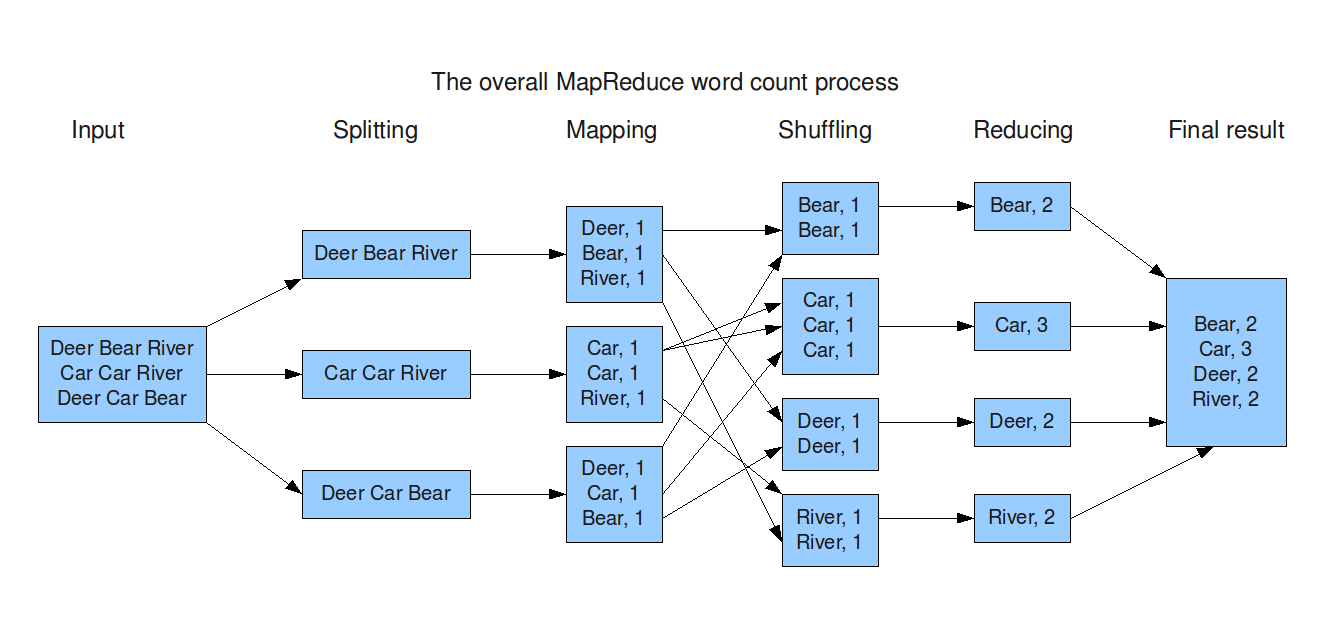
\includegraphics[width=\textwidth]{../images/word_count.png}
\end{frame}

\begin{frame}[fragile]
  \frametitle{Word Count Code}
  wordcounts.py
  \begin{lstlisting}
  from mrjob.job import MRJob
  from string import punctuation

  class MRWordCount(MRJob):
    
      def mapper(self, _, line):
          for word in line.split():
              yield (word.strip(punctuation).lower(), 1)

      def reducer(self, word, counts):
          yield (word, sum(counts))

  if __name__ == '__main__':
      MRWordCount.run()
  \end{lstlisting}

  $\$ : python \;  wordcounts.py \; file/directory \; (> counts.txt) $
\end{frame}

\end{document}
